% -*- LaTeX -*-
% -*- coding: utf-8 -*-
%
% ~~~~~~~~~~~~~~~~~~~~~~~~~~~~~~~~~~~~~~~~~~~~~~~~~~~~~~~~~~~~~~~~~~~~~~~~~~~~~~
%
%                             michael a.g. aïvázis
%                      california institute of technology
%                      (c) 1998-2010  all rights reserved
%
% ~~~~~~~~~~~~~~~~~~~~~~~~~~~~~~~~~~~~~~~~~~~~~~~~~~~~~~~~~~~~~~~~~~~~~~~~~~~~~~
%

\lecture{Overview of parallel systems}{20100108}

% --------------------------------------
% motivation for parallel computing
\begin{frame}[fragile]
%
  \frametitle{Motivations for going parallel}
%
  \begin{itemize}
%
  \item why bother?
    \begin{itemize}
    \item {\em speed}: there are fundamental limits to the processing power of a single processor
    \item {\em throughput}: time to solution is critical for many problems
    \item {\em size}: high resolution requires lots of memory
    \item {\em availability}: the tool exists, use it
    \end{itemize}
%
  \item but be careful
    \begin{itemize}
    \item the commercial market is unstable
    \item the computing environment is somewhat primitive
    \item software packages and libraries are emerging slowly
    \item parallel programming is not hard, but it requires {\em discipline}
    \end{itemize}
%
  \end{itemize}
%
\end{frame}

% --------------------------------------
% computer system taxonomy
\begin{frame}[fragile]
%
  \frametitle{Taxonomy}
%
  \begin{itemize}
%
  \item an early classification of computer systems focused on the relation between {\em
    instruction streams} and {\em data streams}:
    \begin{itemize}
      \item SISD: single instruction, single data
      \item SIMD: single instruction, multiple data
      \item MIMD: multiple instruction, multiple data
    \end{itemize}
%
    \item SISD describes conventional serial computers
    \begin{itemize}
      \item the programming model only: the hardware has moved on...
    \end{itemize}
%
    \item SIMD and MIMD are the traditional models for parallel machines
%
    \item MIMD systems are often programmed in SPMD mode: single {\em program}, multiple data
      \begin{itemize}
      \item when the parallel environment provides a {\em naming scheme} for the instruction
        streams, such as processor id, or task name
      \end{itemize}
  \end{itemize}
%
\end{frame}

% --------------------------------------
% architectural issues
\begin{frame}[fragile]
%
  \frametitle{Architectural issues}
%
  \begin{itemize}
%
  \item {\em control:} SIMD vs.~MIMD
  \item {\em co\"ordination}: synchronous vs.~asynchronous
  \item {\em memory organization}: private vs.~shared
  \item {\em address space}: local vs.~global
  \item {\em memory access}: uniform vs.~non-uniform
  \item {\em granularity}: the power of each processor
  \item {\em scalability}: dependence on the number of processors
  \item {\em interconnect}: topology, routing, switching
%
  \end{itemize}
%
\end{frame}

% --------------------------------------
% tradeoffs
\begin{frame}[fragile]
%
  \frametitle{Tradeoffs}
%
  \begin{center}
    \begin{minipage}{.75\linewidth}
      \begin{tabular}{l|l|l}
                        & shared memory & distributed memory \\ \hline
        scalability     & {\em harder}  & {\em easier} \\
        programmability & {\em easier}  & {\em harder}
      \end{tabular}
    \end{minipage}
  \end{center}

%
  \begin{itemize}
%
  \item shared memory permits parallelizing serial program gradually, focusing on worst
    bottlenecks first
%
  \item distributed memory requires partitioning and distributing both data and work across
    processors, which usually rules out incremental parallelization
%
  \end{itemize}
%
\end{frame}

% --------------------------------------
% categories of parallel architectures
\begin{frame}[fragile]
%
  \frametitle{Categories of parallel architectures}
%
  \begin{itemize}
%
  \item vector or array processor
  \item SMP: symmetric multiprocessor
  \item MPP: massively parallel multiprocessor
  \item DSM: distributed shared memory
  \item clusters
  \item hybrids
    \begin{itemize}
      \item SMP or MPP with vector processors
      \item networked clusters of SMPs
      \item SMP+GPGPU 
    \end{itemize}
%
  \end{itemize}
%
\end{frame}

% --------------------------------------
% generic parallel architecture
\begin{frame}[fragile]
%
  \frametitle{Generic parallel architecture}
%
  \begin{figure}
    \centering
    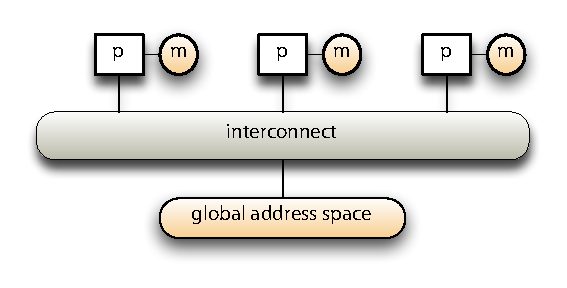
\includegraphics[width=.75\linewidth]{figures/generic-parallel-architecture.pdf}
    \label{fig:generic-parallel-architecture}
  \end{figure}

  \begin{itemize}
%
  \item a trivial but powerful observation: access to memory implies access to information
  \item hence, it becomes a determining factor for both hardware and algorithm design
%
  \end{itemize}
%
\end{frame}

% --------------------------------------
% memory hierarchy
\begin{frame}[fragile]
%
  \frametitle{Memory hierarchy}
%
  \begin{itemize}
  \item high performance architectures have a multi-tier memory hierarchy
%
    \begin{itemize}
    \item registers
    \item on-chip caches, usually referred to as level 1
    \item off-chip caches (level 2)
    \item random access memory
    \item remote memory (off processor)
    \item virtual memory, known as paging memory, that usually involves secondary storage
    \item secondary storage (disks)
    \item tertiary storage (tapes)
    \end{itemize}
%
  \item these have latencies and bandwidths that vary by orders of magnitude
  \item {\em cache misses} are the most frequently cited reason why real codes only achieve a
    small fraction of the benchmarked performance of a CPU
    \begin{itemize}
    \item really small: 10\% of peak is considered a success!
    \end{itemize}
%
  \end{itemize}
%
\end{frame}

% --------------------------------------
% parallel programming paradigms
\begin{frame}[fragile]
%
  \frametitle{Parallel programming paradigms}
%
  \begin{itemize}
%
  \item {\em functional languages}: specify what to compute, not how
  \item {\em parallelizing compilers}: automatic or semi-automatic detection of parallelism in
    serial code; mostly loop-unrolling, often with the help of special mark up (pragmas)
  \item {\em object oriented}: parallelism encapsulated within distributed objects

  \item {\em data parallel}: simultaneous operations on memory; mostly arrays
  \item {\em shared memory}: multiple threads executing a pool of tasks using common memory
  \item {\em remote memory access}: one sided put/get communication between processes
  \item {\em message passing}: two sided, co\"ordinated send/receive communication between
    processes
%
  \end{itemize}
%
\end{frame}

% --------------------------------------
% designing parallel algorithms
\begin{frame}[fragile]
%
  \frametitle{Designing parallel algorithms}
%
  \begin{itemize}
%
  \item {\em identification}: identify the part of the problem that can be parallelized
  \item {\em partition}: decompose the parallelizable part into fine-grained tasks
  \item {\em communication}: determine the necessary communication patterns among tasks
  \item {\em coarsening}: combine into coarser tasks and adjust the communication patterns
  \item {\em task mapping}: assign tasks to processors
%
  \end{itemize}
%
\end{frame}

% --------------------------------------
% paradigms for parallel algorithms
\begin{frame}[fragile]
%
  \frametitle{Paradigms for parallel algorithms}
%
  \begin{itemize}
%
  \item {\em embarrassingly parallel}: mostly independent tasks
  \item {\em functional decomposition}: based on computational task (activity)
  \item {\em data parallel}: aka {\em loop-level} parallelism: array operations
  \item {\em domain decomposition}: based on the distribution of data
  \item {\em divide-and-conquer}: tree-like partitioning
  \item {\em pipelining}: multiple overlapping stages
%
  \end{itemize}
%
\end{frame}

% --------------------------------------
% communication issues
\begin{frame}[fragile]
%
  \frametitle{Communication issues}
%
  \begin{itemize}
%
  \item latency and bandwidth
  \item routing and switching -- not much of an issue any more
  \item contention, flow control and aggregate bandwidth
  \item collective communication
    \begin{itemize}
      \item one to many: broadcast, scatter
      \item many to one: gather, reduction, scan
      \item all to all
      \item synchronization barrier
    \end{itemize}
  \item assigning work to processors
    \begin{itemize}
    \item partitioning
    \item granularity
    \item mapping
    \item scheduling
    \item load balancing
    \end{itemize}
%
  \end{itemize}
%
\end{frame}

% --------------------------------------
% performance factors
\begin{frame}[fragile]
%
  \frametitle{Factors determining performance}
%
  \begin{itemize}
%
  \item {\em concurrency}: maximize the work that can be done in parallel
  \item {\em load balance}: make sure the load is (and stays) divided evenly
  \item {\em parallel overhead}: work not present in the equivalent serial computation
    \begin{itemize}
      \item process startup and shutdown costs
      \item communication
      \item synchronization
      \item redundancy
      \item speculative work
    \end{itemize}
%
  \end{itemize}
%
\end{frame}

% --------------------------------------
% computational models
\begin{frame}[fragile]
%
  \frametitle{Computational models}
%
  \begin{itemize}
%
    \item abstractions for architecture, algorithm analysis, and performance modeling
      \begin{itemize}
      \item PRAM: Parallel random access machine
      \item LogP: latency, overhead, gap, processors
      \item BSP: bulk synchronous parallel
      \item CSP: communicating sequential processes
      \item ... and many others
      \end{itemize}
%
    \item all occasionally useful tools for reasoning about implementation strategies for real
      programs, since they steer you away from common but perhaps non-obvious mistakes
    \item unfortunately, none is a substitute for understanding the characteristics of your
      target platform
%
  \end{itemize}
%
\end{frame}

% end of file 
